%% Creator: Inkscape inkscape 0.48.5, www.inkscape.org
%% PDF/EPS/PS + LaTeX output extension by Johan Engelen, 2010
%% Accompanies image file 'subrot.pdf' (pdf, eps, ps)
%%
%% To include the image in your LaTeX document, write
%%   \input{<filename>.pdf_tex}
%%  instead of
%%   \includegraphics{<filename>.pdf}
%% To scale the image, write
%%   \def\svgwidth{<desired width>}
%%   \input{<filename>.pdf_tex}
%%  instead of
%%   \includegraphics[width=<desired width>]{<filename>.pdf}
%%
%% Images with a different path to the parent latex file can
%% be accessed with the `import' package (which may need to be
%% installed) using
%%   \usepackage{import}
%% in the preamble, and then including the image with
%%   \import{<path to file>}{<filename>.pdf_tex}
%% Alternatively, one can specify
%%   \graphicspath{{<path to file>/}}
%% 
%% For more information, please see info/svg-inkscape on CTAN:
%%   http://tug.ctan.org/tex-archive/info/svg-inkscape
%%
\begingroup%
  \makeatletter%
  \providecommand\color[2][]{%
    \errmessage{(Inkscape) Color is used for the text in Inkscape, but the package 'color.sty' is not loaded}%
    \renewcommand\color[2][]{}%
  }%
  \providecommand\transparent[1]{%
    \errmessage{(Inkscape) Transparency is used (non-zero) for the text in Inkscape, but the package 'transparent.sty' is not loaded}%
    \renewcommand\transparent[1]{}%
  }%
  \providecommand\rotatebox[2]{#2}%
  \ifx\svgwidth\undefined%
    \setlength{\unitlength}{1200bp}%
    \ifx\svgscale\undefined%
      \relax%
    \else%
      \setlength{\unitlength}{\unitlength * \real{\svgscale}}%
    \fi%
  \else%
    \setlength{\unitlength}{\svgwidth}%
  \fi%
  \global\let\svgwidth\undefined%
  \global\let\svgscale\undefined%
  \makeatother%
  \begin{picture}(1,0.36666667)%
    \put(0,0){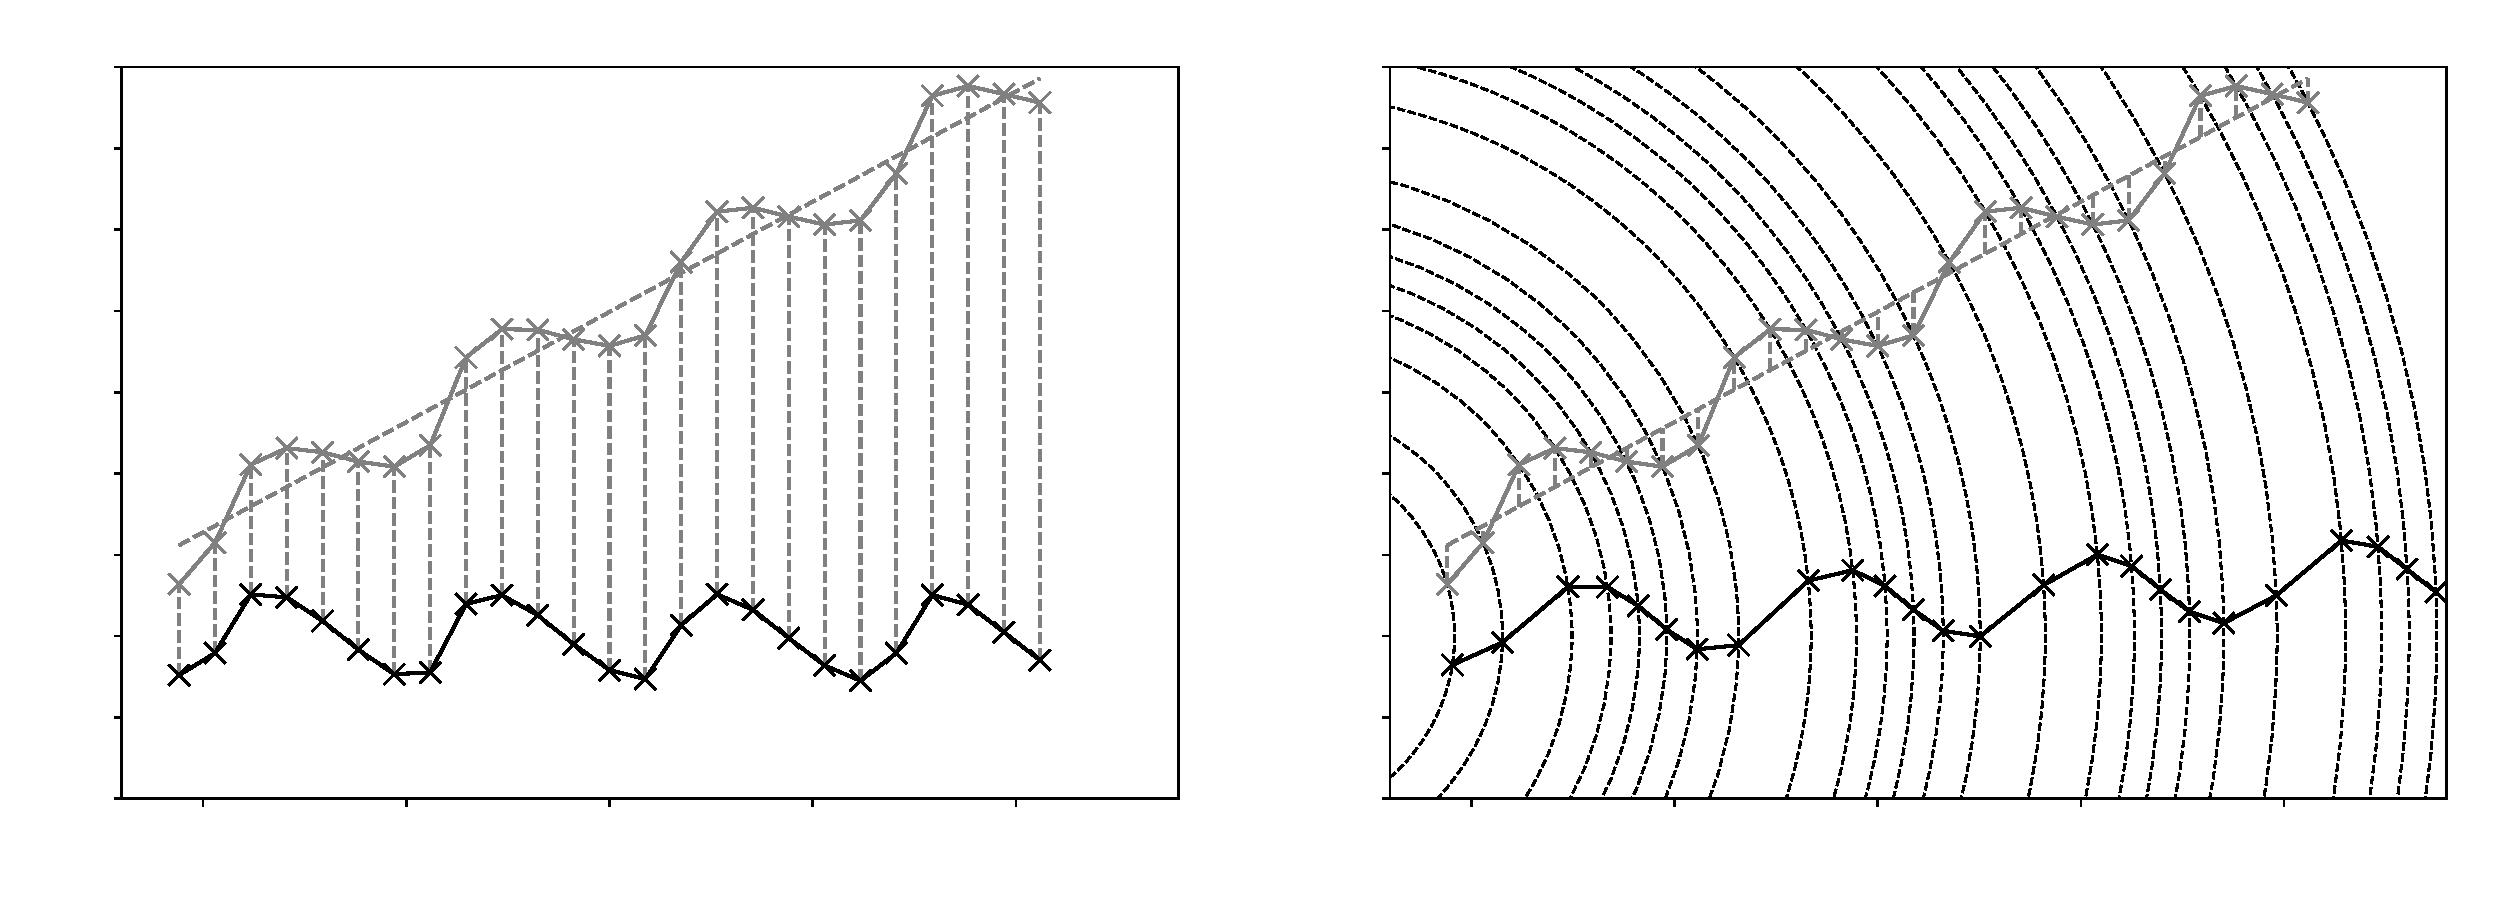
\includegraphics[width=\unitlength]{subrot.pdf}}%
    \put(0.08120764,0.03513659){\makebox(0,0)[b]{\smash{5}}}%
    \put(0.16250135,0.03513659){\makebox(0,0)[b]{\smash{10}}}%
    \put(0.24379506,0.03513659){\makebox(0,0)[b]{\smash{15}}}%
    \put(0.32508875,0.03513659){\makebox(0,0)[b]{\smash{20}}}%
    \put(0.40638247,0.03513659){\makebox(0,0)[b]{\smash{25}}}%
    \put(0.26005379,0.02373812){\makebox(0,0)[b]{\smash{Coordinates (a.u.)}}}%
    \put(0.04285683,0.04413592){\makebox(0,0)[rb]{\smash{−4}}}%
    \put(0.04285683,0.07665342){\makebox(0,0)[rb]{\smash{−2}}}%
    \put(0.04285683,0.10917089){\makebox(0,0)[rb]{\smash{0}}}%
    \put(0.04285683,0.14168836){\makebox(0,0)[rb]{\smash{2}}}%
    \put(0.04285683,0.17420585){\makebox(0,0)[rb]{\smash{4}}}%
    \put(0.04285683,0.20672333){\makebox(0,0)[rb]{\smash{6}}}%
    \put(0.04285683,0.23924082){\makebox(0,0)[rb]{\smash{8}}}%
    \put(0.04285683,0.27175829){\makebox(0,0)[rb]{\smash{10}}}%
    \put(0.04285683,0.30427578){\makebox(0,0)[rb]{\smash{12}}}%
    \put(0.04285683,0.33679326){\makebox(0,0)[rb]{\smash{14}}}%
    \put(0.02550528,0.19363062){\rotatebox{90}{\makebox(0,0)[b]{\smash{Heights (a.u.)}}}}%
    \put(0.26005379,0.34495928){\makebox(0,0)[b]{\smash{Subtraction}}}%
    \put(0.58848035,0.03513659){\makebox(0,0)[b]{\smash{5}}}%
    \put(0.66977409,0.03513659){\makebox(0,0)[b]{\smash{10}}}%
    \put(0.75106773,0.03513659){\makebox(0,0)[b]{\smash{15}}}%
    \put(0.83236152,0.03513659){\makebox(0,0)[b]{\smash{20}}}%
    \put(0.91365516,0.03513659){\makebox(0,0)[b]{\smash{25}}}%
    \put(0.76732653,0.02373812){\makebox(0,0)[b]{\smash{Coordinates (a.u.)}}}%
    \put(0.55012957,0.04413592){\makebox(0,0)[rb]{\smash{−4}}}%
    \put(0.55012957,0.07665342){\makebox(0,0)[rb]{\smash{−2}}}%
    \put(0.55012957,0.10917089){\makebox(0,0)[rb]{\smash{0}}}%
    \put(0.55012957,0.14168836){\makebox(0,0)[rb]{\smash{2}}}%
    \put(0.55012957,0.17420585){\makebox(0,0)[rb]{\smash{4}}}%
    \put(0.55012957,0.20672333){\makebox(0,0)[rb]{\smash{6}}}%
    \put(0.55012957,0.23924082){\makebox(0,0)[rb]{\smash{8}}}%
    \put(0.55012957,0.27175829){\makebox(0,0)[rb]{\smash{10}}}%
    \put(0.55012957,0.30427578){\makebox(0,0)[rb]{\smash{12}}}%
    \put(0.55012957,0.33679326){\makebox(0,0)[rb]{\smash{14}}}%
    \put(0.532778,0.1936306){\rotatebox{90}{\makebox(0,0)[b]{\smash{Heights (a.u.)}}}}%
    \put(0.76732653,0.34495928){\makebox(0,0)[b]{\smash{Rotation}}}%
  \end{picture}%
\endgroup%
